\documentclass{article}
\usepackage[top=1in, bottom=1in, left=1in, right=1in]{geometry}
\usepackage{amsmath,cite}
\usepackage{graphicx}
\usepackage{subcaption}
\usepackage{times, epsfig, graphicx,url, bm}
\usepackage{amssymb}
\usepackage{epstopdf}
\usepackage{tikz}
\usetikzlibrary{bayesnet}

\DeclareMathOperator*{\argmax}{arg\,max}


% Title.
% ------
\title{Dictionary Prior $\mathrm{P}(\mathbf{W})$}
\author{
Dawen Liang \\
\texttt{daliang@adobe.com}
} \date{}

\begin{document}
%
\maketitle
%

\section{Source-filter model (version 1)}
\begin{figure}[ht]
  \centering
      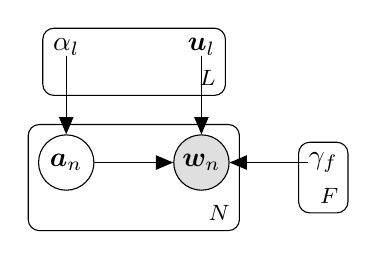
\begin{tikzpicture}

  % Define nodes
  \node[obs] 			(w) {$\bm{w}_n$};
  \node[const, right=of w] (s) {${\gamma}_f$};
  \node[latent, left=of w] (a) {$\bm{a}_n$};
  \node[const, above=of w] (u) {$\bm{u}_l$};
  \node[const, above=of a] (alpha) {$\alpha_l$};

  % Connect the nodes
  \edge {a} {w} ; %
  \edge {s} {w};
  \edge {u} {w};
  \edge {alpha}{a};

  % Plates
  \plate {wa} {(w)(a)} {$N$};
  \plate {au} {(alpha)(u)} {$L$};
  \plate {sigma} {(s)} {$F$};

\end{tikzpicture}

  \caption{Version 1}
\label{fig:plate}
\end{figure}

Model formulation:
\[
\bm{w}_t \in \mathbb{R}_{+}^{F} \qquad \bm{a}_t \in \mathbb{R}_{+}^{L} \qquad \bm{u}_l  \in \mathbb{R}_{+}^{F}\\
\]
\begin{align*}
a_{tl} &\sim \Gamma(\alpha_l, \alpha_l)\\
\log {w}_{tf} &\sim \mathcal{N}(\sum_{l=1}^L a_{tl} u_{lf}, 1/\gamma_f)
\end{align*}

Objective:
\begin{align*}
\hat{\mathbf{U}}, \hat{\bm{\alpha}}, \hat{\bm{\gamma}} &= \argmax_{\mathbf{U}, \bm{\alpha}, \bm{\gamma}} \sum_t \log P(\bm{w}_t | \mathbf{U}, \bm{\alpha}, \bm{\gamma})\\
&= \argmax_{\mathbf{U}, \bm{\alpha}, \bm{\gamma}} \sum_t \log \int_{\bm{a}_t} P(\bm{w}_t, \bm{a}_t | \mathbf{U}, \bm{\alpha}, \bm{\gamma}) \mathrm{d} \bm{a}_t
\end{align*}


\section{Variational EM:}
\subsection{E-step}
\begin{itemize}
\item Reparametrize $v_{tf} \equiv \log w_{tf}$ and $\phi_{tl} \equiv \log a_{tl}$.
\item Approximate posterior $P(\bm{a}_t | \mathbf{U}, \bm{w}_t, \bm{\alpha}, \bm{\gamma}) = \prod_{l} q(a_{tl})$.
\end{itemize}

\subsubsection{Laplace Approximation:} 

\begin{align*}
q(a_{tl}) &\propto \exp \{ (\alpha_l - 1) \log a_{tl} - \alpha_l a_{tl} - \frac{1}{2} \sum_f \gamma_f  \langle (v_{tf} - \sum_k a_{tk} u_{kf})^2 \rangle \}\\
\Rightarrow q(\phi_{tl}) &\propto \exp \biggl\{ \alpha_l  \phi_{tl}  + \exp(\phi_{tl}) \biggl(\sum_f \gamma_f u_{lf} \hat{v}_{tf}^{-l} - \alpha_l\biggl) - \frac{1}{2} \exp(2\phi_{tl}) \sum_f \gamma_f u_{lf}^2  \biggl\}\\
&= \exp\{f(\phi_{tl})\}
\end{align*}
where 
\[
\hat{v}_{tf}^{-l} = v_{tf} - \sum_{k\neq l} \langle \exp(\phi_{tk})\rangle u_{kf}
\]

Search for the local maximum $\hat{\phi}_{tl}$ of $f(\phi_{tl})$:
\begin{align*}
\mu_{tl} &\leftarrow \hat{\phi}_{tl}\\
\sigma_{tl}^2 & \leftarrow -\biggl(\frac{\partial^2 f } {\partial \phi_{tl}^2} (\hat{\phi}_{tl})\biggl)^{-1}
\end{align*}

\subsubsection{Directly optimizing variational bound}

 The variational bound is:
\begin{align*}
\mathcal{L}=& \sum_t \biggl\{  \langle \log P(\bm{w}_t, \bm{a}_t | \mathbf{U}, \bm{\alpha}, \bm{\gamma}) \rangle + \sum_l H_q (a_{tl}) \biggl\}
\end{align*}
where
\begin{align*}
 \langle \log P(\bm{w}_t, \bm{a}_t | \mathbf{U}, \bm{\alpha}, \bm{\gamma}) \rangle  \propto & \sum_f \langle -\frac{1}{2} \gamma_f (v_{tf} - \sum_k a_{tk} u_{kf})^2 \rangle + \sum_l  (\alpha_l - 1) \langle \log a_{tl} \rangle - \alpha_l \langle a_{tl} \rangle
\end{align*}

Depending on which variational distribution we choose to use, $H_q(a_{tl})$ can take on different forms. If $q(\log a_{tl}) = \mathcal{N}(\mu_{tl}, \sigma_{tl}^2)$: 
\begin{align*}
H_q (a_{tl}) \propto \frac{1}{2}\log ( \sigma_{tl}^2) + \mu_{tl}
\end{align*}
else if $q(a_{tl}) = \Gamma(k_{tl}, \mu_{tl})$ (a gamma distribution with shape $k_{tl}$ and mean $\mu_{tl}$):
\begin{align*}
H_q (a_{tl}) = k_{tl} - \log \biggl(\frac{k_{tl}}{\mu_{tl}}\biggl) + \log \Gamma(k_{tl}) + (1 - k_{tl})\psi(k_{tl})
\end{align*}
Furthermore,
\begin{align*}
& \sum_f \langle -\frac{1}{2} \gamma_f (v_{tf} - \sum_k a_{tk} u_{kf})^2 \rangle \\
\propto & \sum_f \frac{1}{2} \gamma_f \biggl\{ 2 v_{tf} \sum_k \langle a_{tk} \rangle u_{kf} -  \langle \big(\sum_k a_{tk} u_{kf}\big)^2 \rangle \biggl\}
\end{align*}

All the expectations can be computed as:
\begin{center}
\begin{tabular} { c || c | c }
& $q(\log a_{tl}) = \mathcal{N}(\mu_{tl}, \sigma_{tl}^2)$ & $q(a_{tl}) = \Gamma(k_{tl}, \mu_{tl})$ \\ \hline
$\langle a_{tl} \rangle$  & $\exp(\mu_{tl} + \frac{1}{2} \sigma_{tl}^2)$ & $\mu_{tl}$ \\ \hline
$\langle a_{tl}^2 \rangle$ & $\exp(2\mu_{tl} + 2\sigma_{tl}^2)$ & $\mu_{tl}^2 + \frac{\mu_{tl}^2}{k_{tl}}$\\ \hline
$\langle \log a_{tl} \rangle$ & $\mu_{tl}$ & $\psi(k_{tl}) - \log \biggl( \frac{k_{tl}}{\mu_{tl}} \biggl)$ \\
\end{tabular}
\end{center}

Therefore, we can optimize $\mathcal{L}$ with respect to variational parameters for $l\in [L]$. The objective function is:
\begin{align*}
\mathcal{L}_l
\propto \sum_t \biggl\{ \langle a_{tl} \rangle (\sum_f \gamma_f u_{lf} \hat{v}_{tf}^{-l} -\alpha_l) - \frac{1}{2} \langle a_{tl}^2 \rangle \sum_f \gamma_f u_{lf}^2
+ (\alpha_l - 1) \langle \log a_{tl} \rangle  + H_q(a_{tl}) \biggl\} 
\end{align*}
The gradient of $\mathcal{L}_l$ under log-normal variational distribution: 
\[
\frac{\partial \mathcal{L}_l}{\partial \mu_{tl}} = \langle a_{tl} \rangle (\sum_f \gamma_f u_{lf} \hat{v}_{tf}^{-l} - \alpha_l) - \langle a_{tl}^2 \rangle \sum_f \gamma_f u_{lf}^2  + \alpha_l  
\]
\[
\frac{\partial \mathcal{L}_l}{\partial (\sigma^2_{tl})} = \frac{1}{2} \langle a_{tl} \rangle  (\sum_f \gamma_f u_{lf} \hat{v}_{tf}^{-l} - \alpha_l) - \langle a_{tl}^2 \rangle \sum_f \gamma_f  u_{lf}^2 + \frac{1}{2\sigma_{tl}^2}
\]
The gradient of $\mathcal{L}_l$ under gamma variational distribution: 
\[
\frac{\partial \mathcal{L}_l}{\partial k_{tl}} = \frac{\mu_{tl}^2}{2 k^2_{tl}}  \sum_f \gamma_f  u_{lf}^2 + (\alpha_l - k_{tl}) \psi_1(k_{tl}) - \frac{\alpha_l}{k_{tl}} + 1
\]
\[
\frac{\partial \mathcal{L}_l}{\partial \mu_{tl}} =  (\sum_f \gamma_f u_{lf} \hat{v}_{tf}^{-l} - \alpha_l) - (\mu_{tl} + \frac{\mu_{tl}}{k_{tl}})\sum_f \gamma_f u_{lf}^2 + \frac{\alpha_l}{\mu_{tl}}
\]
While doing optimization, L-BFGS can be adopted. Note that since we are alternating across independent directions $l \in [L]$, multiple sweeps are required until convergence. On the other hand, we can optimize $\mathcal{L}$ for $t \in [T]$ which can be done via L-BFGS only once. The objective function is:
\begin{align*}
\mathcal{L}_t 
\propto  \sum_f \frac{1}{2} \gamma_f \biggl\{ 2 v_{tf} \sum_k \langle a_{tk} \rangle u_{kf} -  \langle \big(\sum_k a_{tk} u_{kf}\big)^2 \rangle \biggl\}
+ \sum_l \biggl\{(\alpha_l - 1) \langle \log a_{tl} \rangle  - \alpha_l \langle a_{tl} \rangle \biggl\} + \sum_l H_q (a_{tl})
\end{align*}
The elements of gradient for $\mathcal{L}_t$ are essentially the same as the corresponding ones of $\mathcal{L}_l$.

\subsection{M-step:}

The objective function for M-step is:
\begin{align*}
\mathcal{L}(\mathbf{U}, \bm{\alpha}, \bm{\gamma}) &= \sum_t \langle \log P(\bm{w}_t, \bm{a}_t | \mathbf{U}, \bm{\alpha}, \bm{\gamma}) \rangle \\
&\propto \sum_t  \biggl\{ \frac{1}{2}\sum_f \langle \log \gamma_f - \gamma_f (v_{tf} - \sum_k a_{tk} u_{kf})^2 \rangle + \sum_l \langle \alpha_l \log \alpha_l - \log \Gamma(\alpha_l) + (\alpha_l - 1)\log a_{tl} - \alpha_l a_{tl}  \rangle \biggl\}
\end{align*}

Take the derivative w.r.t. $\mathbf{U}, \bm{\alpha}, \bm{\gamma}$, respectively:
\begin{align*}
\frac{\partial \mathcal{L}}{\partial u_{lf}} &\propto \sum_t \biggl( \langle a_{tl} \rangle \hat{v}_{tf}^{-l} - \langle a_{tl}^2 \rangle u_{lf} \biggl)\\
\frac{\partial \mathcal{L}}{\partial \alpha_l} &\propto  \sum_t \biggl( \log \alpha_l + 1 - \psi(\alpha_l) + \langle \log a_{tl} \rangle - \langle a_{tl} \rangle \biggl)\\
\frac{\partial \mathcal{L}}{\partial \gamma_f} &\propto \sum_t \frac{1}{\gamma_f} -  \biggl(v_{tf}^2 - 2 v_{tf}  \sum_k \langle a_{tk} \rangle u_{kf} +  \langle (\sum_k a_{tk} u_{kf})^2 \rangle \biggl)
\end{align*}
where
\begin{align*}
\langle (\sum_k a_{tk} u_{kf})^2 \rangle = \sum_k \langle a_{tk}^2 \rangle u_{kf}^2 + (\sum_k \langle a_{tk} \rangle u_{kf})^2 - \sum_k \langle a_{tk}\rangle ^2 u_{kf}^2
\end{align*}

Note that for $\gamma_f$, closed form update is available:
\begin{equation*}
\gamma_f^{-1} = \frac{1}{T}\sum_t \biggl(v_{tf}^2 - 2 v_{tf}  \sum_k \langle a_{tk} \rangle u_{kf} +  \langle (\sum_k a_{tk} u_{kf})^2 \rangle \biggl)
\end{equation*}

While for $U$ and $\alpha$, L-BFGS can be applied to find a local optimum. Note that since $\alpha_l > 0$ which can be problematic for numerical solver, we log-transform $\eta_l \equiv \log \alpha_l$ and optimize w.r.t. $\eta_l$, where the derivative can be simply modified by chain rule:
\[
\frac{\partial \mathcal{L}}{\partial \eta_l} = \frac{\partial \mathcal{L}}{\partial \alpha_l} \cdot \frac{\partial \alpha_l}{\partial \eta_l} = \alpha_l \frac{\partial \mathcal{L}}{\partial \alpha_l} 
\]

\section{Gamma noise model}

To better adopt for NMF setting, it would be appropriate to model $\bm{w}_t$ with a gamma noise model instead of a log-normal noise model:
\[
w_{tf} \sim \Gamma\Big(\gamma_f, \gamma_f  \prod_l \exp(-a_{tl} u_{lf})\Big)
\]
and keep the rest of the model unchanged. The variational distribution in this setting is $q(a_{tl}) = \Gamma(k_{tl}, \beta_{tl})$ which is a gamma distribution with shape $k_{tl}$ and rate $\beta_{tl}$. Directly optimizing the variational bound:
\begin{align*}
\mathcal{L}_t=&  \langle \log P(\bm{w}_t, \bm{a}_t | \mathbf{U}, \bm{\alpha}, \bm{\gamma}) \rangle + \sum_l H_q (a_{tl})
\end{align*}
where
\begin{align*}
 \langle \log P(\bm{w}_t, \bm{a}_t | \mathbf{U}, \bm{\alpha}, \bm{\gamma}) \rangle  \propto & \sum_f \gamma_f \biggl\{-w_{tf} \prod_{l} \langle \exp(-a_{tl} u_{lf}) \rangle - \sum_l \langle a_{tl} \rangle u_{lf} \biggl\}  + \sum_l  \biggl\{ (\alpha_l - 1) \langle \log a_{tl} \rangle - \alpha_l \langle a_{tl} \rangle \biggl\}
\end{align*}

All the expectations can be computed as:
\begin{center}
\begin{tabular} { c || c  }
& $q(a_{tl}) = \Gamma(k_{tl}, \beta_{tl})$ \\ \hline
$\langle a_{tl} \rangle$  &  $\frac{k_{tl}}{\beta_{tl}}$ \\ \hline
$\langle \exp(-a_{tl}u_{lf} \rangle$ & $(1 + \frac{u_{lf}}{\beta_{tl}})^{-k_{tl}}$ if $\beta_{tl} > -u_{lf}$, $+\infty$ otherwise.\\ \hline
$\langle \log a_{tl} \rangle$ & $\psi(k_{tl}) - \log \beta_{tl}$ \\
\end{tabular}
\end{center}

Take the derivative of $\mathcal{L}_t$ w.r.t. $k_{tl}$ and $\beta_{tl}$:
\begin{align*}
\frac{\partial \mathcal{L}_t}{\partial k_{tl}} &= \sum_f \biggl\{ w_{tf} \gamma_f \log(1 + \frac{u_{lf}}{\beta_{tl}}) \prod_{k} \langle \exp(-a_{tk} u_{kf}) \rangle - \gamma_f \frac{u_{lf}}{\beta_{tl}} \biggl\} + (\alpha_l - k_{tl}) \psi_1(k_{tl}) + 1 - \frac{\alpha_l}{\beta_{tl}}\\
\frac{\partial \mathcal{L}_t}{\partial \beta_{tl}} &= \frac{k_{tl}}{\beta_{tl}^2} \sum_f \biggl\{ -w_{tf} \gamma_f (1 + \frac{u_{lf}}{\beta_{tl}})^{-1} u_{lf} \prod_{k} \langle \exp(-a_{tk} u_{kf}) \rangle + \gamma_f u_{lf} \biggl\} + \alpha_l (\frac{k_{tl}}{\beta_{tl}^2} - \frac{1}{\beta_{tl}})
\end{align*}

\subsection{M-step}
The objective function for M-step is:
\begin{align*}
\mathcal{L}(\mathbf{U}, \bm{\alpha}, \bm{\gamma}) &= \sum_t \langle \log P(\bm{w}_t, \bm{a}_t | \mathbf{U}, \bm{\alpha}, \bm{\gamma}) \rangle \\
&= \sum_t  \biggl\{ \sum_f \Big( \gamma_f \log \gamma_f - \gamma_ f \sum_l \langle a_{tl} \rangle u_{lf} - \log\Gamma(\gamma_f) + (\gamma_f - 1)\log w_{tf} - w_{tf} \gamma_f \prod_l \langle \exp(-a_{tl} u_{lf}) \rangle \Big)  \\
&+ \sum_l  \Big( \alpha_l \log \alpha_l - \log \Gamma(\alpha_l) + (\alpha_l - 1)\langle \log a_{tl} \rangle - \alpha_l \langle a_{tl}  \rangle \Big) \biggl\}
\end{align*}

Take the derivative w.r.t. $\mathbf{U}, \bm{\alpha}, \bm{\gamma}$, respectively:
\begin{align*}
\frac{\partial \mathcal{L}}{\partial u_{lf}} &= \sum_t \biggl( - \langle a_{tl} \rangle + w_{tf} \langle a_{tl} \rangle (1 + \frac{u_{lf}}{\beta_{tl}})^{-(k_{tl}+1)}  \prod_{k \neq l} \langle \exp(-a_{tk} u_{kf}) \rangle \biggl)\\
\frac{\partial \mathcal{L}}{\partial \alpha_l} &=  \sum_t \biggl( \log \alpha_l + 1 - \psi(\alpha_l) + \langle \log a_{tl} \rangle - \langle a_{tl} \rangle \biggl)\\
\frac{\partial \mathcal{L}}{\partial \gamma_f} &= \sum_t \biggl( \log \gamma_f - \sum_l \langle a_{tl} \rangle u_{lf} + 1 - \psi(\gamma_f) + \log w_{tf} - w_{tf} \prod_l \langle \exp(-a_{tl} u_{lf}) \rangle \biggl)
\end{align*}

\section{Full NMF model}
\begin{figure}[ht]
  \centering
      % model_pca.tex
%
% Copyright (C) 2012 Jaakko Luttinen
%
% This file may be distributed and/or modified
%
% 1. under the LaTeX Project Public License and/or
% 2. under the GNU General Public License.
%
% See the files LICENSE_LPPL and LICENSE_GPL for more details.

% PCA model

%\beginpgfgraphicnamed{model-pca}
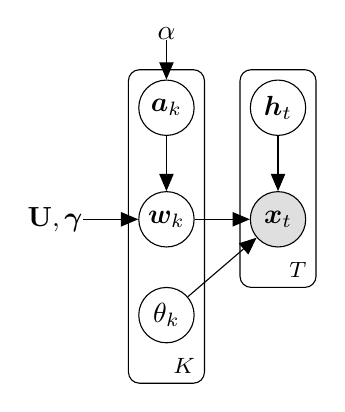
\begin{tikzpicture}

  % Define nodes
\node[obs] 			(x) {$\bm{x}_t$};
\node[latent, above=0.7cm of x]   (h) {$\bm{h}_t$};
\node[latent, left=0.7cm of x]       (w) {$\bm{w}_k$};
\node[latent, below=0.5cm of w]  (t)  {$\theta_k$};
\node[latent, above=0.7cm of w]  (a) {$\bm{a}_k$};
\node[const, above=0.5cm of a]  (alpha) {$\alpha$};
\node[const, left=0.7cm of w]      (u)  {$\mathbf{U, \bm{\gamma}}$};

  % Connect the nodes
\edge {h} {x};
\edge {w} {x};
\edge {t} {x};
\edge {a} {w};
\edge {alpha} {a};
\edge {u} {w};

  % Plates
  %\plate {yx} {(x)(y)} {$N$} ;
%  \plate {wa} {(w)(a)} {$T$};
%  \plate {au} {(alpha)(u)} {$L$};
%  \plate {sigma} {(s)} {$F$};
  %\plate {} {(d)(y)(yx.north west)(yx.south west)} {$T$} ;
\plate {hx} {(x)(h)} {$T$};
\plate {twa} {(t)(w)(a)} {$K$};

\end{tikzpicture}
%\endpgfgraphicnamed


  \caption{Full NMF model}
\label{fig:plate}
\end{figure}

Model formulation:
\begin{align*}
a_{lk} &\sim \Gamma(\alpha_l, \alpha_l)\\
W_{fk} &\sim \Gamma\Big(\gamma_f, \gamma_f \prod_l \exp(-U_{fl} a_{lk})\Big)\\
H_{kt} &\sim \Gamma(b, b)\\
\theta_k &\sim \Gamma(\beta/K, c)\\
X_{ft} &\sim \text{Exp}\Big(\sum_k \theta_k W_{fk} H_{kt}\Big)\\
\biggl(\text{or } X_{ft} &\sim \text{Poisson}\Big(\sum_k \theta_k W_{fk} H_{kt}\Big)\biggl)
\end{align*}

Let's begin with GaP-NMF.


\end{document}
